%%% ===============================================================================
\chapter{Design and Implementation}\label{sec:design}
%%% ===============================================================================
\section{RDF Authoring Panel}\label{sec:design:rdf-authoring-panel}

The \gls{rdf} authoring functionality is implemented as a dedicated, separate panel in MetaConfigurator, located in \texttt{meta\_configurator/src/components/panels/rdf}. This design keeps semantic authoring concerns modular while still integrating with the existing session, path selection, and data editing flow of MetaConfigurator \cite{metaconfigurator2024}. At runtime, the entry component \texttt{RdfPanel.vue} validates whether the current data can be treated as \gls{jsonld} and provides immediate warnings for missing \texttt{@context}, invalid syntax, and non-\gls{jsonld} input.

Figure \ref{fig:rdf_authoring_panel:json_data} shows a snapshot of the \gls{rdf} panel in action, loaded with the \gls{json} example from \ref{lst:background_json_example}. Since the data is provided in \gls{json} format, the panel indicates that it must first be converted to \gls{jsonld} before further processing. The user can proceed in two ways: either by directly supplying a \gls{jsonld} document in the text view, or by using the \textbf{JSON-to-JSON-LD} conversion tool discussed in Section \ref{sec:design:rdf-authoring-panel:rml-mapping-tool}.

\begin{figure}
  \centering
  
\includegraphics[width=.65\linewidth]{../figures/MC-RDF-JSON.png}
  \caption{A snapshot of MetaConfigurator's RDF panel.}
    \label{fig:rdf_authoring_panel:json_data}
\end{figure}

\subsection{RML Mapping Tool}
\label{sec:design:rdf-authoring-panel:rml-mapping-tool}

If the input data is not already expressed as \gls{jsonld}, the \gls{rdf} panel provides a conversion tool that enables users to transform \gls{json} data into \gls{rdf}-compatible \gls{jsonld} using \gls{rml} mappings. \gls{rml} extends the \gls{r2rml} mapping language and allows the transformation of heterogeneous data sources such as \gls{json}, \gls{csv}, or \gls{xml} into \gls{rdf} graphs \cite{dimou2014rml}. Figure~\ref{fig:rdf_authoring_panel:rml_1} illustrates the dialog used to define such mappings.

\begin{figure}[htbp]
  \centering
  
\includegraphics[width=.65\linewidth]{../figures/MC-RDF-RML-1.png}
  \caption{The RML mapping dialog for JSON-to-JSON-LD conversion.}
  \label{fig:rdf_authoring_panel:rml_1}
\end{figure}

\begin{figure}[htbp]
  \centering
  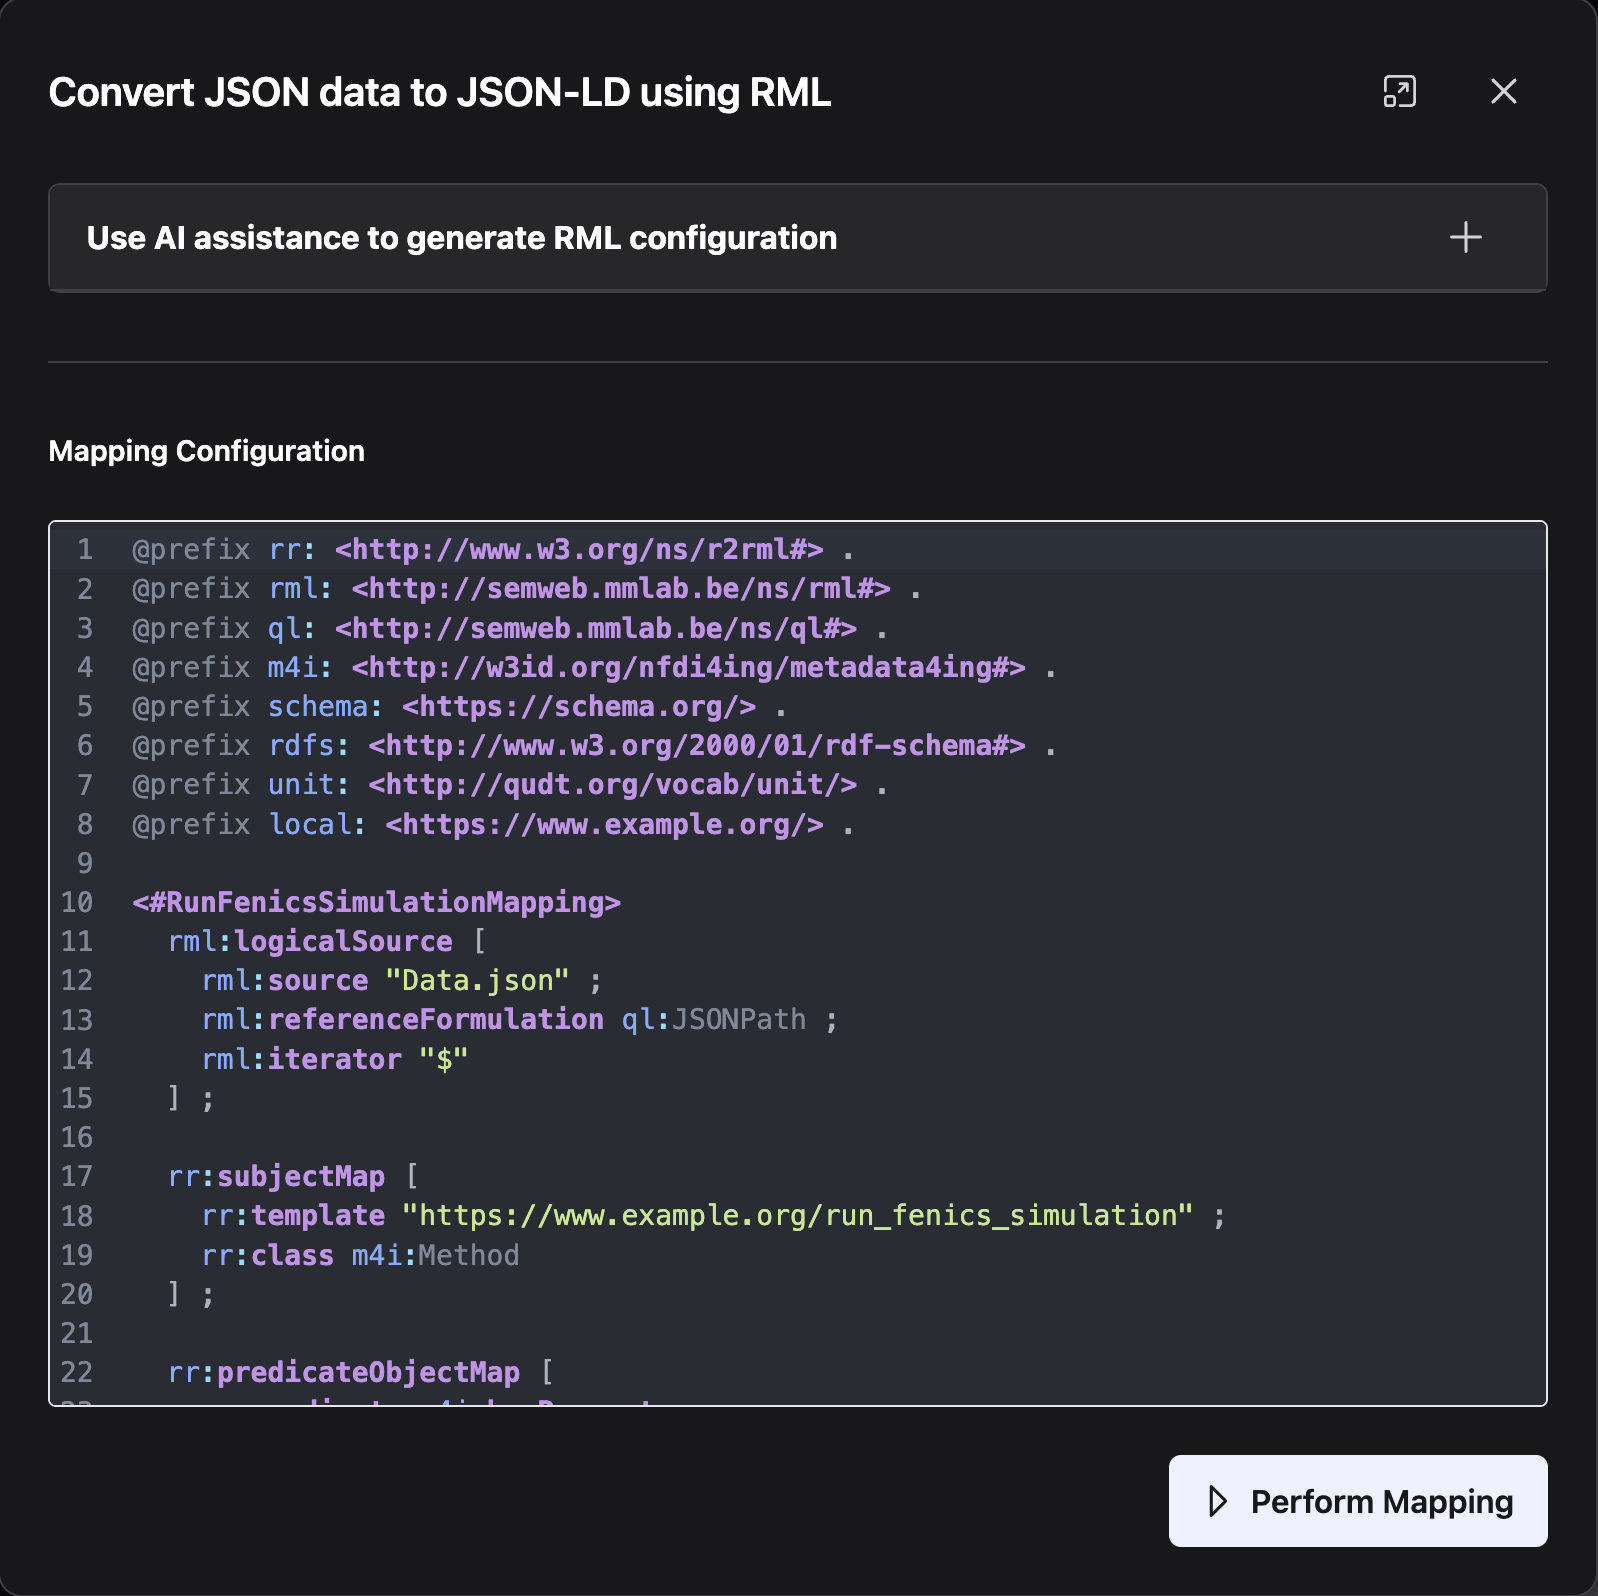
\includegraphics[width=.65\linewidth]{../figures/MC-RDF-RML-2.png}
\caption{AI-generated RML mapping based on user-provided hints from Listing \ref{lst:metaconfigurator_interface_rdf:rml_hint}.}
  \label{fig:rdf_authoring_panel:rml_2}
\end{figure}

The dialog allows users to either provide an existing \gls{rml} mapping or generate one automatically with \gls{ai} assistance. In the latter case, the user supplies mapping hints that describe how elements of the input \gls{json} data should correspond to \gls{rdf} properties or classes. These hints, together with a representative subset of the input data, are sent to an external \gls{ai} API to generate a candidate mapping.

Internally, the system constructs a structured prompt that includes example mappings and fragments of the input data. This prompt guides the language model to produce a valid \gls{rml} mapping in Turtle syntax that conforms to the target \gls{jsonld} structure. The prompt constrains the model to return only the mapping definition while adhering to \gls{rml} rules, thereby improving reliability and syntactic correctness.

The mapping editor is implemented using the CodeMirror component, a widely used web-based code editor that provides syntax highlighting and automatic indentation \cite{codemirror}. Mapping validity is checked by the mapping service through debounced live validation. This allows users to inspect, refine, and validate the generated mapping directly within the interface before applying it to transform the \gls{json} input into \gls{jsonld}.

Users may either provide an \gls{rml} mapping in Turtle syntax directly or use the \gls{ai}-assisted generation feature by supplying mapping hints. The resulting mapping is displayed in the CodeMirror editor, where it can be reviewed and edited as needed. Since the mapping is generated by \gls{ai}, user verification and refinement are recommended. Once finalized, the mapping can be applied to convert the input \gls{json} data into \gls{jsonld}, which can then be further managed in the \gls{rdf} authoring panel.

For example, a sample mapping hint that could convert the \gls{json} example in Listing \ref{lst:background_json_example} to the \gls{jsonld} example in Listing \ref{lst:background_jsonld_example} is depicted in Listing \ref{lst:metaconfigurator_interface_rdf:rml_hint}. This hint describes how to create \gls{rdf} resources for the simulation run, parameters, and metrics, and how to link them using appropriate properties from the \texttt{schema} and \texttt{m4i} vocabularies. It also specifies how to map \gls{json} fields to \gls{rdf} properties, including handling units via the \gls{qudt} vocabulary.

After providing these hints, the configured \gls{ai} model generates an \gls{rml} mapping that follows the specified structure and semantics, as shown in Figure \ref{fig:rdf_authoring_panel:rml_2}. This mapping closely resembles the one presented in Listing \ref{lst:background_rml_mapping}. Once the user reviews and confirms the mapping, it can be executed to transform the input \gls{json} data into a semantically enriched \gls{jsonld} representation, as illustrated in Figure \ref{fig:rdf_authoring_panel:jsonld_1}.

\begin{lstlisting}[style=plaintext,caption={Sample RML hints which describe the mapping from JSON to JSON-LD}, label={lst:metaconfigurator_interface_rdf:rml_hint}]
Create one main resource local:run_fenics_simulation of type m4i:Method.
This node links to parameter nodes using m4i:hasParameter and to metric nodes using m4i:investigates.

Iterate over the arrays parameters[*] and metrics[*] separately to create parameter and metric nodes.

For each entry in these arrays:

Create a resource with IRI local:variable_{name} using the "name" field.
Set the type to schema:PropertyValue.
Set rdfs:label to the "name" value.
Set schema:value to the "value" field using rml:reference.
Map the "unit" field to schema:unitCode as an IRI from the QUDT unit vocabulary using the template http://qudt.org/vocab/unit/{unit}.

Connect the method node to parameter nodes using m4i:hasParameter, and to metric nodes using m4i:investigates.

Use these prefixes in the mapping:
m4i: http://w3id.org/nfdi4ing/metadata4ing#
schema: https://schema.org/
rdfs: http://www.w3.org/2000/01/rdf-schema#
unit: http://qudt.org/vocab/unit/
local: https://www.example.org/
\end{lstlisting}


\begin{figure}
  \centering
  
\includegraphics[width=.65\linewidth]{../figures/MC-RDF-JSON-LD-2.png}
  \caption{JSON-LD output obtained by applying the mapping from Listing \ref{lst:background_rml_mapping}, focused on the Context tab.}
  \label{fig:rdf_authoring_panel:jsonld_2}
\end{figure}

\begin{figure}
  \centering
  
\includegraphics[width=.65\linewidth]{../figures/MC-RDF-JSON-LD-1.png}
  \caption{JSON-LD output obtained by applying the mapping from Listing \ref{lst:background_rml_mapping}, focused on the Triples tab.}
  \label{fig:rdf_authoring_panel:jsonld_1}
\end{figure}

\subsection{Panel Composition and UI Structure}

The core editing surface is implemented in \texttt{RdfEditorPanel.vue} as a PrimeVue Tabs\footnote{\url{https://primevue.org/tabs/}} container. The implementation is primarily organized into two tabs:
\begin{itemize}
    \item \textbf{Context tab}: for editing \texttt{@context} definitions.
    \item \textbf{Triples tab}: for browsing and editing \gls{rdf} triples.
\end{itemize}

This explicit split mirrors the conceptual separation in \gls{jsonld} between vocabulary declarations and graph assertions \cite{jsonld2014}. The panel therefore supports both semantic modeling tasks (namespace/prefix handling) and graph authoring tasks (subject-predicate-object manipulation) in one workflow.

\subsection{Context Tab Implementation}

The Context tab is implemented by \texttt{RdfContextEditorPanel.vue}. It reuses MetaConfigurator's \gls{gui} editor and applies a predefined JSON Schema so that \texttt{@context} can be edited through structured forms rather than plain text only. The selection updates are synchronized with the text editor view, enabling users to navigate to and manipulate context entries consistently with other panels.

When the current document is invalid or not in the expected \gls{jsonld} form, both tabs become visually disabled. This prevents accidental modifications when parsing preconditions are not satisfied.

\subsection{Triples Tab Implementation}

The Triples tab is implemented by \texttt{RdfTripleEditorPanel.vue}. It presents triples in a PrimeVue \texttt{DataTable} \footnote{\url{https://primevue.org/datatable/}} with:
\begin{itemize}
    \item paging, sorting, and column/global filtering,
    \item single-row selection synchronized with document path selection in the text editor,
    \item actions for add, edit, delete, export, \gls{sparql}, and visualization.
\end{itemize}

Triple editing is handled through \texttt{TripleDetailsDialog.vue}, which allows controlled entry of subject, predicate, and object terms, including typed literals with XML Schema datatypes. Changes are executed through \texttt{TripleEditorService} and propagated to the central \gls{rdf} store.

Data changes occur from two sources: the JSON text editor and the triples DataTable. When a change is made in the JSON editor, \texttt{rdfStoreManager.ts} rebuilds the \gls{rdf} graph and updates the triples view (Figure \ref{fig:rdf_authoring_panel:change_propagation_json_editor}).

Conversely, when a triple is edited, removed, or added in the DataTable, \texttt{TripleEditorService} validates and applies the change through \texttt{rdfStoreManager.ts}. If successful, \texttt{jsonLdNodeManager.ts} rebuilds \gls{jsonld} from the updated store and writes it back to the Data Editor state, which updates the text view accordingly (Figure \ref{fig:rdf_authoring_panel:change_propagation_rdf_view}).

\begin{figure}[htbp]
  \centering
  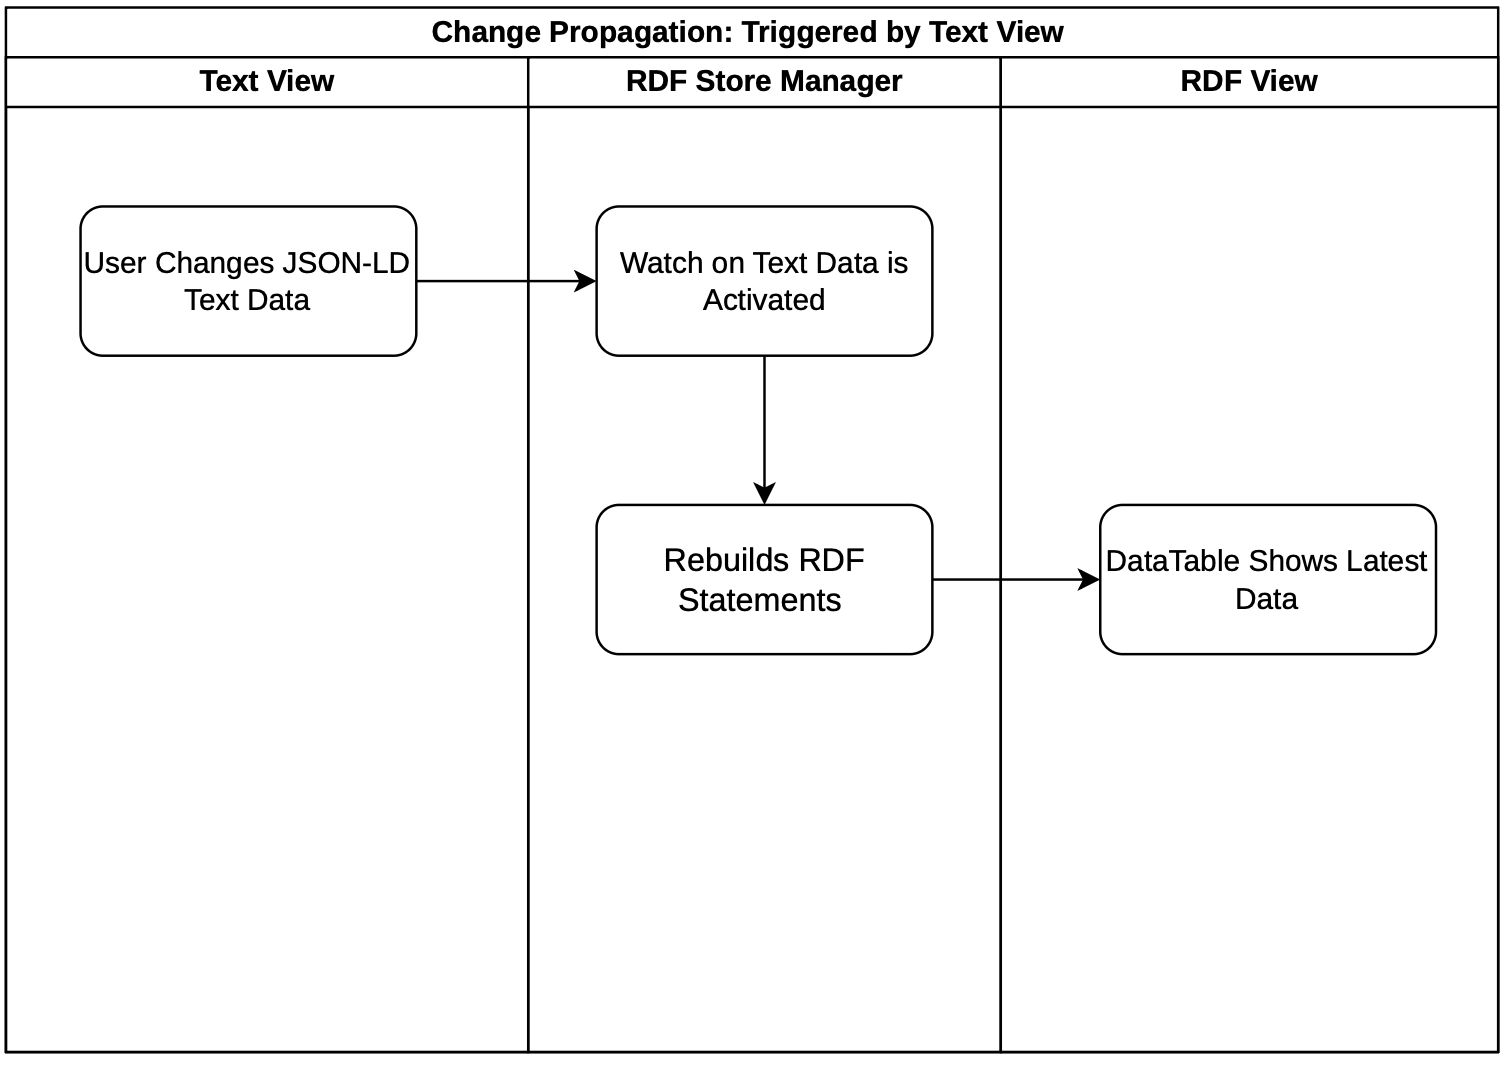
\includegraphics[width=.65\linewidth]{../figures/Diagram-1.png}
  \caption{Change propagation flow between Text View and RDF View when the source of change is the Text View.}
  \label{fig:rdf_authoring_panel:change_propagation_json_editor}
\end{figure}

\begin{figure}[htbp]
  \centering
  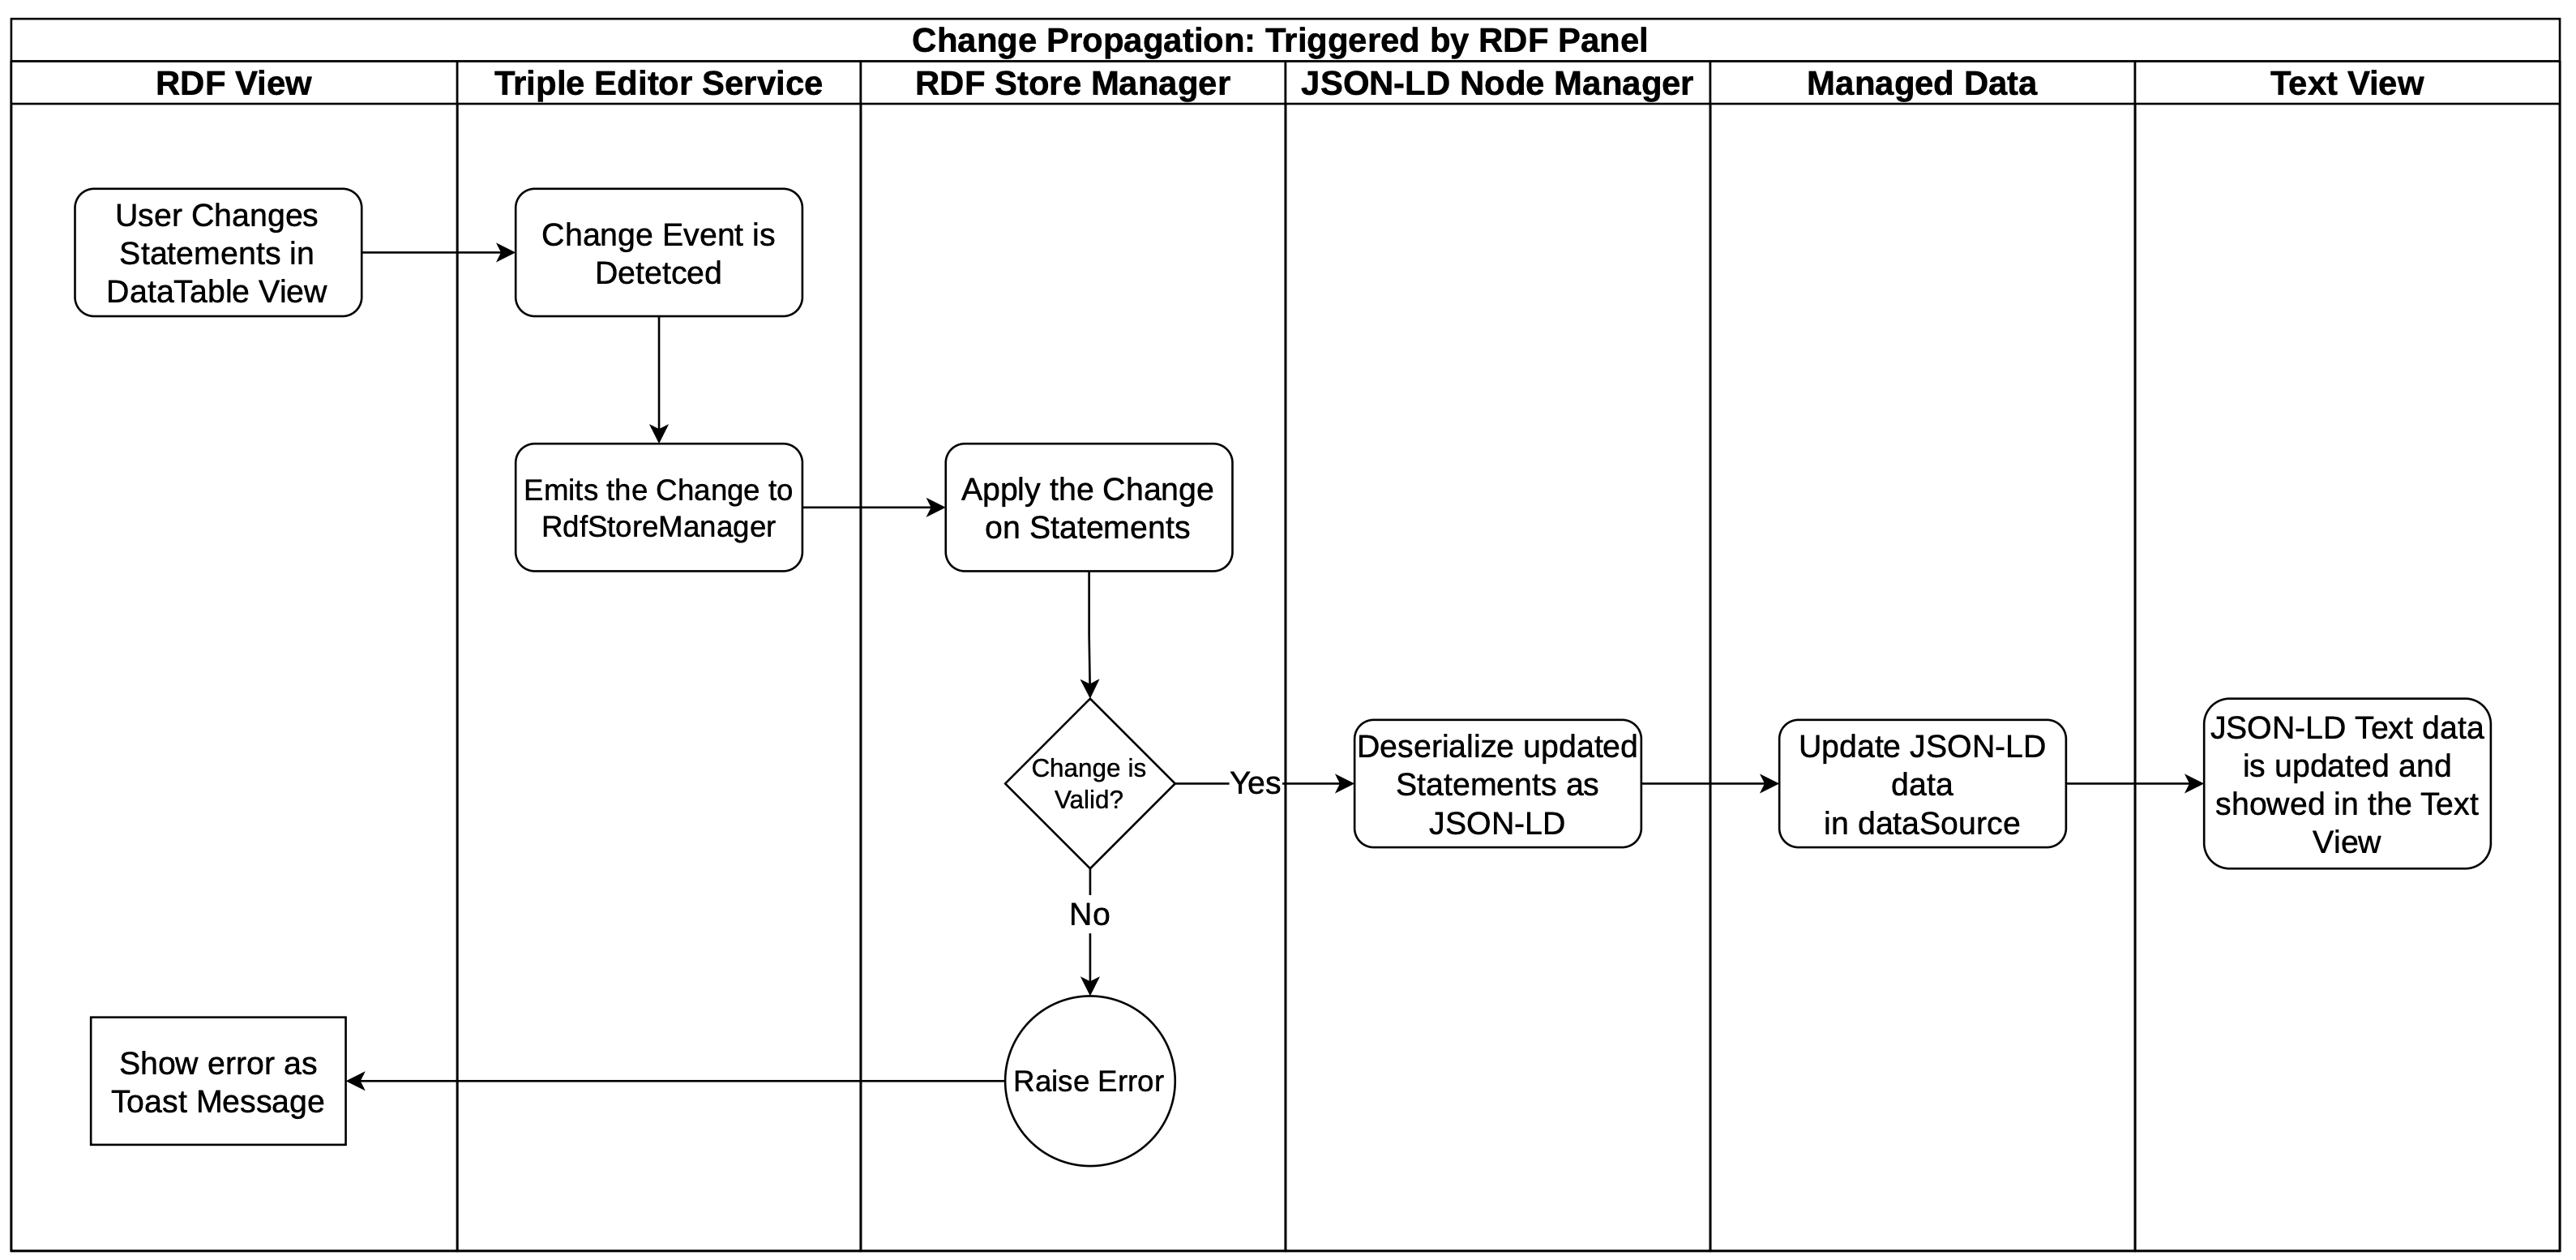
\includegraphics[width=.65\linewidth]{../figures/Diagram-2.png}
  \caption{Change propagation flow between Text View and RDF View when the source of change is the RDF View.}
  \label{fig:rdf_authoring_panel:change_propagation_rdf_view}
\end{figure}

\subsection{RDF Store and Data Synchronization}

The internal semantic state is managed by \texttt{rdfStoreManager.ts}, which uses RDFLib to parse and serialize data \cite{rdflib_docs}. On each source-data update, the manager:
\begin{enumerate}
    \item resolves \texttt{@context} data into namespace mappings,
    \item parses \gls{jsonld} into an indexed \gls{rdf} graph and derives a reactive list of Statements,
    \item exposes reactive Statements, warnings, and errors to UI components.
\end{enumerate}

\begin{definition}[RDFLib Statement]
In this implementation, an RDFLib Statement is the runtime representation of one \gls{rdf} triple of the form $(s, p, o)$, where $s$ (subject), $p$ (predicate), and $o$ (object) are \gls{rdf} terms. In \texttt{rdflib.js}, these terms are represented as \texttt{NamedNode}, \texttt{BlankNode}, and \texttt{Literal} objects, and each triple is stored as a \texttt{\$rdf.Statement}. A collection of such statements forms the in-memory graph used by the panel \cite{rdflib_docs}.

\end{definition}

This definition is directly reflected in the implementation workflow: \texttt{rdfStoreManager.ts} parses \gls{jsonld} into a list of \texttt{\$rdf.Statement} objects (\texttt{statements.value}), \texttt{RdfTripleEditorPanel.vue} renders this list in the Data Table, and \texttt{TripleEditorService} creates or modifies individual statements for add/edit/delete operations. Statement-level matching (subject, predicate, object) functions are usedto synchronize table selection with text-editor paths.

To keep the \gls{json} editor and \gls{rdf} authoring panel consistent, \texttt{jsonLdNodeManager.ts} maps \gls{rdf} statements back into \gls{jsonld} data and computes path correspondences between selected triples and document positions. This enables bidirectional synchronization: selecting a triple can focus the matching JSON path, and raw \gls{json} data changes trigger store rebuilds.

\subsection{Integrated Extensions in the Triple Workflow}

The Triple tab also integrates two advanced features:
\begin{itemize}
    \item \textbf{SPARQL dialog} (\texttt{SparqlEditor.vue}): query execution and result inspection aligned with SPARQL standards \cite{sparql_standard}.
    \item \textbf{Graph visualization} (\texttt{RdfVisualizer.vue}): interactive inspection of currently filtered triples as a graph representation.
\end{itemize}

Together, this implementation turns the RDF panel into a full authoring environment: users can define context terms, curate triples, run semantic queries, and visually inspect graph structures in a single, cohesive interface.



\section{Query with SPARQL}\label{sec:design:query-with-sparql}
\section{Knowledge Graph Visualization}\label{sec:design:knowledge-graph-visualization}
